\section{Převodníky AD typu SAR a integrační}
- základní zapojení a funkce, příklady využití.

\subsection{SAR}
Kompenzační převodníky AD s postupnou aproximací obsahují řídicí obvod převodníku konstruovaný pro postupnou aproximaci (SAR) měřeného napětí u\textsubscript{VST} vhodně volenými kroky rekonstrukčního napětí u\textsubscript{DAC}. Převodník tedy srovnává vstupní napětí postupně s napětími odpovídajícími jednotlivým váhám, nejvyšší váhou (MSB) počínaje a nejmenší (LSB) konče.
\begin{figure}[h]
   \begin{center}
     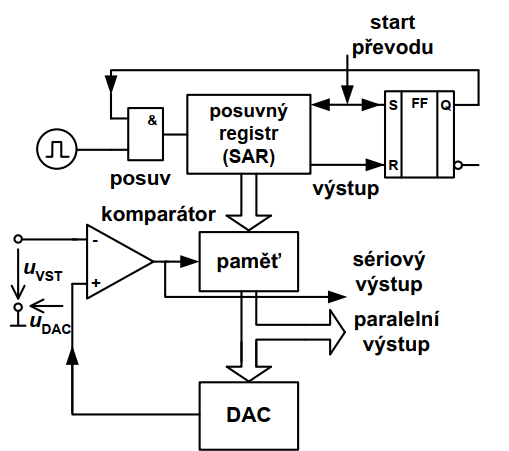
\includegraphics[scale=0.6]{images/ADCkomp.png}
   \end{center}
   \caption{Kompenzační ADC s postupnou aproximací}
\end{figure}

Převod se začíná zápisem 1 do posuvného registru na pozici nejvyššího bitu. Tato 1 se v dalších krocích posouvá po všech bitech n–bitového slova C. Tím se postupně přidávají jednotlivá váhová napětí a komparují se se vstupním napětím převodníku. Podle reakce komparátoru se na dané pozici bitu jednička i v dalších krocích ponechá (když u\textsubscript{VST} > u\textsubscript{DAC}) nebo se nahradí nulou (když bylo už u\textsubscript{VST} $\leq$ u\textsubscript{DAC}). Pro libovolně velké vstupní napětí z povoleného rozsahu uVST $\in$ $<$ 0; UM) probíhá převod v n–bitovém převodníku vždy právě v n taktech.

Na b) je pro názornost uveden grafický průběh ustalování rekonstrukčního napětí u\textsubscript{DAC} pro převod vstupního napětí u\textsubscript{VST} blízkého minimálnímu napětí rozsahu ADC. Princip je stále stejný, výsledkem je dvojkové číslo 00000010.
\begin{figure}[h]
   \begin{center}
     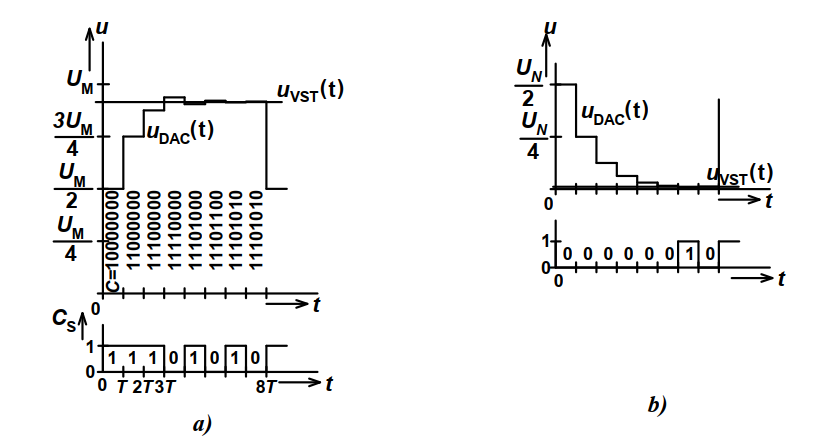
\includegraphics[scale=0.6]{images/dia.png}
   \end{center}
   \caption{Časový diagram převodu s postupnou aproximací a) pro velké u\textsubscript{VST}, b) pro malé
u\textsubscript{VST}}
\end{figure}

Tento typ převodníku se vyrábí v hybridní i monolitické podobě, snadno se sestavuje z jednotlivých integrovaných bloků, popř. se velmi snadno sestaví kombinací mikropočítače, napěťového komparátoru a rekonstrukčního převodníku DA.

\subsubsection{ADC s postupnou aproximací a vyrovnáváním náboje}
Tento převodník je tvořen soustavou kapacitorů s váhově odstupňovanými kapacitami C, 2C, 4C atd. V režimu vzorkování jsou horní elektrody kapacitorů připojeny na napětí U\textsubscript{L} = 0 V a spodní elektrody na měřené vstupní napětí U\textsubscript{x}. V režimu vzorkování se kapacitory nabíjí na napětí rozdílu U\textsubscript{x} a U\textsubscript{L}.

V režimu pamatování se elektronické přepínače přepnou tak, že se horní elektrody odpojí od U\textsubscript{L} a naopak spodní elektrody se na U\textsubscript{L} připojí.
\begin{figure}[h]
   \begin{center}
     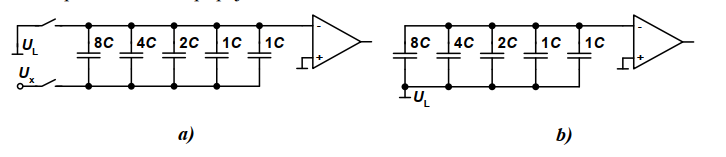
\includegraphics[scale=0.6]{images/ADprox.png}
   \end{center}
   \caption{Funkce převodníku s postupnou aproximací a vyrovnáváním náboje}
\end{figure}
\begin{figure}[h]
   \begin{center}
     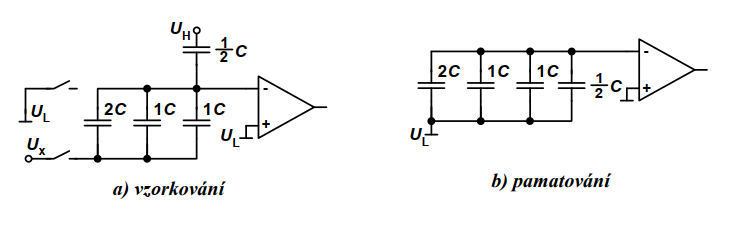
\includegraphics[scale=0.6]{images/ADprox3.png}
   \end{center}
   \caption{Metoda posunu převodní charakteristiky}
\end{figure}

\pagebreak
V režimu postupné aproximace se počínaje MSB kapacitory postupně přepínají z U\textsubscript{L} = 0 na U\textsubscript{H}. Výstupní signál komparátoru potom určí, zda v dalším kroku zůstane spodní elektroda připojena na U\textsubscript{H} nebo se vrátí do U\textsubscript{L} = 0.
\begin{figure}[h]
   \begin{center}
     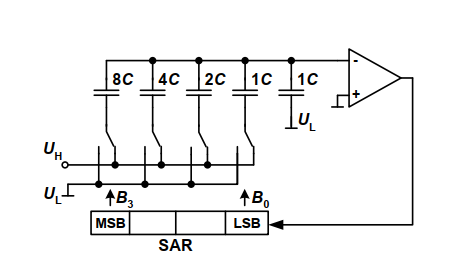
\includegraphics[scale=0.6]{images/ADprox2.png}
   \end{center}
   \caption{Funkce převodníku s postupnou aproximací a vyrovnáváním náboje}
\end{figure}


\begin{figure}[h]
   \begin{center}
     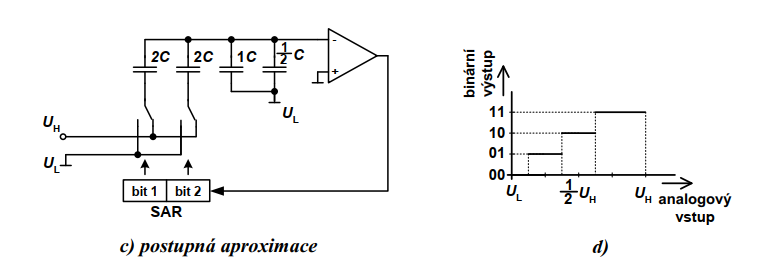
\includegraphics[scale=0.6]{images/ADprox4.png}
   \end{center}
   \caption{Metoda posunu převodní charakteristiky}
\end{figure}

\newpage
\subsection{Integrační převodníky AD}
Integrační převodníky AD používají princip integrace vstupního napětí a mezipřevodu doby integrace na výstupní číslicový signál. Převodníky lze dělit na převodníky s mezipřevodem na kmitočet a s mezipřevodem na šířku impulzu. Základní stavební jednotkou těchto převodníků AD je přepínaný integrátor.

\subsubsection{Integrační převodník AD s mezipřevodem na kmitočet}
\begin{figure}[h]
   \begin{center}
     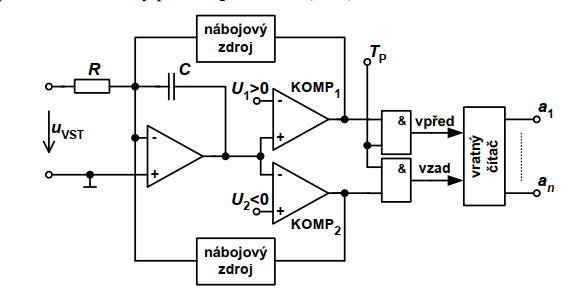
\includegraphics[scale=0.6]{images/ADint.png}
   \end{center}
   \caption{Princip zapojení integračního převodníku ADC s mezipřevodem na kmitočet}
\end{figure}

Vstupní napětí u\textsubscript{VST} je integrováno po dobu:
\begin{equation}
T_{i}=\frac{U_{R}}{u_{vst}}*RC
\end{equation}
,za kterou výstupní napětí zesilovače dosáhne komparační úrovně U1 > 0.

Kmitočet f překlápění komparátoru určuje za předpokladu T\textsubscript{ref} $\rightarrow$ 0 hodnotu:
\begin{equation}
f=\frac{1}{T_{1}}=\frac{u_{vst}}{U_{ref}*RC}
\end{equation}

Pro vstupní napětí opačné polarity pracuje obdobně větev s druhým komparátorem. U konkrétních realizací je nábojový zdroj tvořen monostabilním klopným obvodem, který po přesně definovanou dobu spíná analogový spínač, připojující referenční napětí k rezistoru, jímž pak protéká definovaný proud I podle:
\begin{equation}
Q_{1}=-I*T_{ref}=-c*U_{ref}
\end{equation}

\subsubsection{Integrační převodník ADC s mezipřevodem na časový interval}
Jde o typ s dvojsklonnou integrací, který proti základnímu typu s jednosklonnou integrací má řadu výhod. Odstraňuje vliv nestability rezistoru a kapacitoru v integračním zesilovači a nestability kmitočtu z pomocného generátoru. Převodník v prvním
kroku integruje vstupní napětí a ve druhém kroku referenční napětí. Příchodem startovacího impulzu na vstup S se klopný obvod KO\textsubscript{1} na výstupu Q nastaví a sepne spínač S\textsubscript{1}. Integrátor integruje vstupní napětí u\textsubscript{VST} po dobu:
\begin{equation}
T_{1}=\frac{2^n}{f}
\end{equation}

určenou naplněním čítače s kapacitou 2\textsuperscript{n} impulzy s kmitočtem f z pomocného generátoru, které procházejí přes otevřené hradlo H\textsubscript{1}. Na konci prvního kroku bude výstupní napětí integrátoru:
\begin{equation}
u_{i}(T_{1})=u_{vst}*\frac{T_{1}}{RC}
\end{equation}
Po naplnění čítače se jeho signálem přeplnění vynuluje klopný obvod KO\textsubscript{1} a spínač S\textsubscript{1} se rozpojí. Naopak se nastaví klopný obvod KO\textsubscript{2}, z jehož výstupu se ovládá spínač S\textsubscript{2}, který připojí na vstup integrátoru záporné referenční napětí U\textsubscript{ref} < 0. Čítač nyní čítá impulzy z generátoru přes otevřené hradlo H\textsubscript{2}. Integrátor integruje referenční napětí po dobu T\textsubscript{2}, danou dosažením nulové hodnoty výstupního napětí u\textsubscript{i}. Jakmile výstupní napětí integrátoru projde nulou, signalizuje tuto situaci komparátor a vynuluje klopný obvod KO\textsubscript{2}. Signálem z jeho výstupu se rozpojí spínač S\textsubscript{2} a uzavře hradlo H\textsubscript{2}.
\begin{figure}[h]
   \begin{center}
     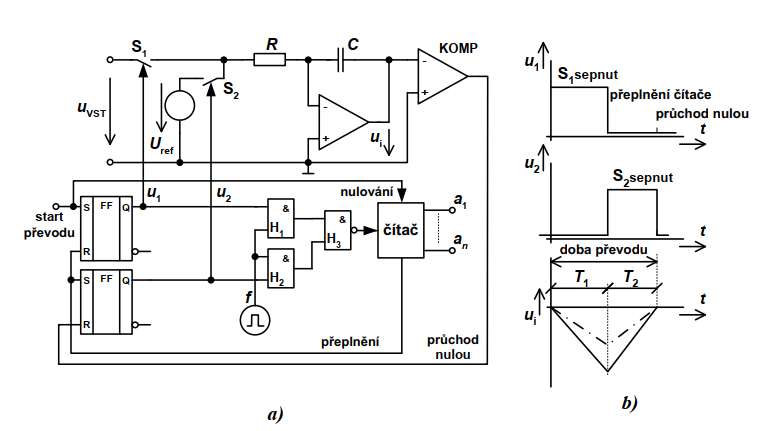
\includegraphics[scale=0.6]{images/ADdvoj.png}
   \end{center}
   \caption{K principu činnosti převodníku ADC s dvojsklonnou integrací}
\end{figure}

\pagebreak
Přesnost převodu uvažovaného typu převodníku nezávisí na dlouhodobé stabilitě integračního rezistoru R a kapacitoru C. Při změně časové konstanty RC se pouze změní směrnice časových průběhů napětí u\textsubscript{i} , avšak doba T\textsubscript{2} zůstane konstantní.

Rychlost převodu s dvojsklonnou integrací je možné zvýšit, rozdělí-li se časový interval integrace referenčního napětí na dva časové úseky, přičemž strmost výstupního napětí integrátoru je v prvním úseku integrace referenčního napětí větší než ve druhém.










